\chapter{Appendices}
\label{ch:appendices}

\todo{Finish writing in-text appendices; this is just a placeholder chapter}

For more detailed discussion of methods that doesn't make a key contribution to the main text of the thesis.

\section{Acknowledgements}
The long list of people who helped in some way.

Family, Supervisors, Northern Synod people (esp. Steve Orme and Daphne Reade),
my Yolngu and other Indigenous friends who encouraged me (esp. Rronang);
the BOM for supplying data, CSIRO people who gave their time,
the academic and professional staff of the Fenner school,


\section{Human Ethics Approval} \label{sec:ethics}
Everything related to ethics approval, including letter of invitation etc.

There must be a standard form of words for this; reference approval number etc.

\begin{figure}[p]
    \centering
    \frame{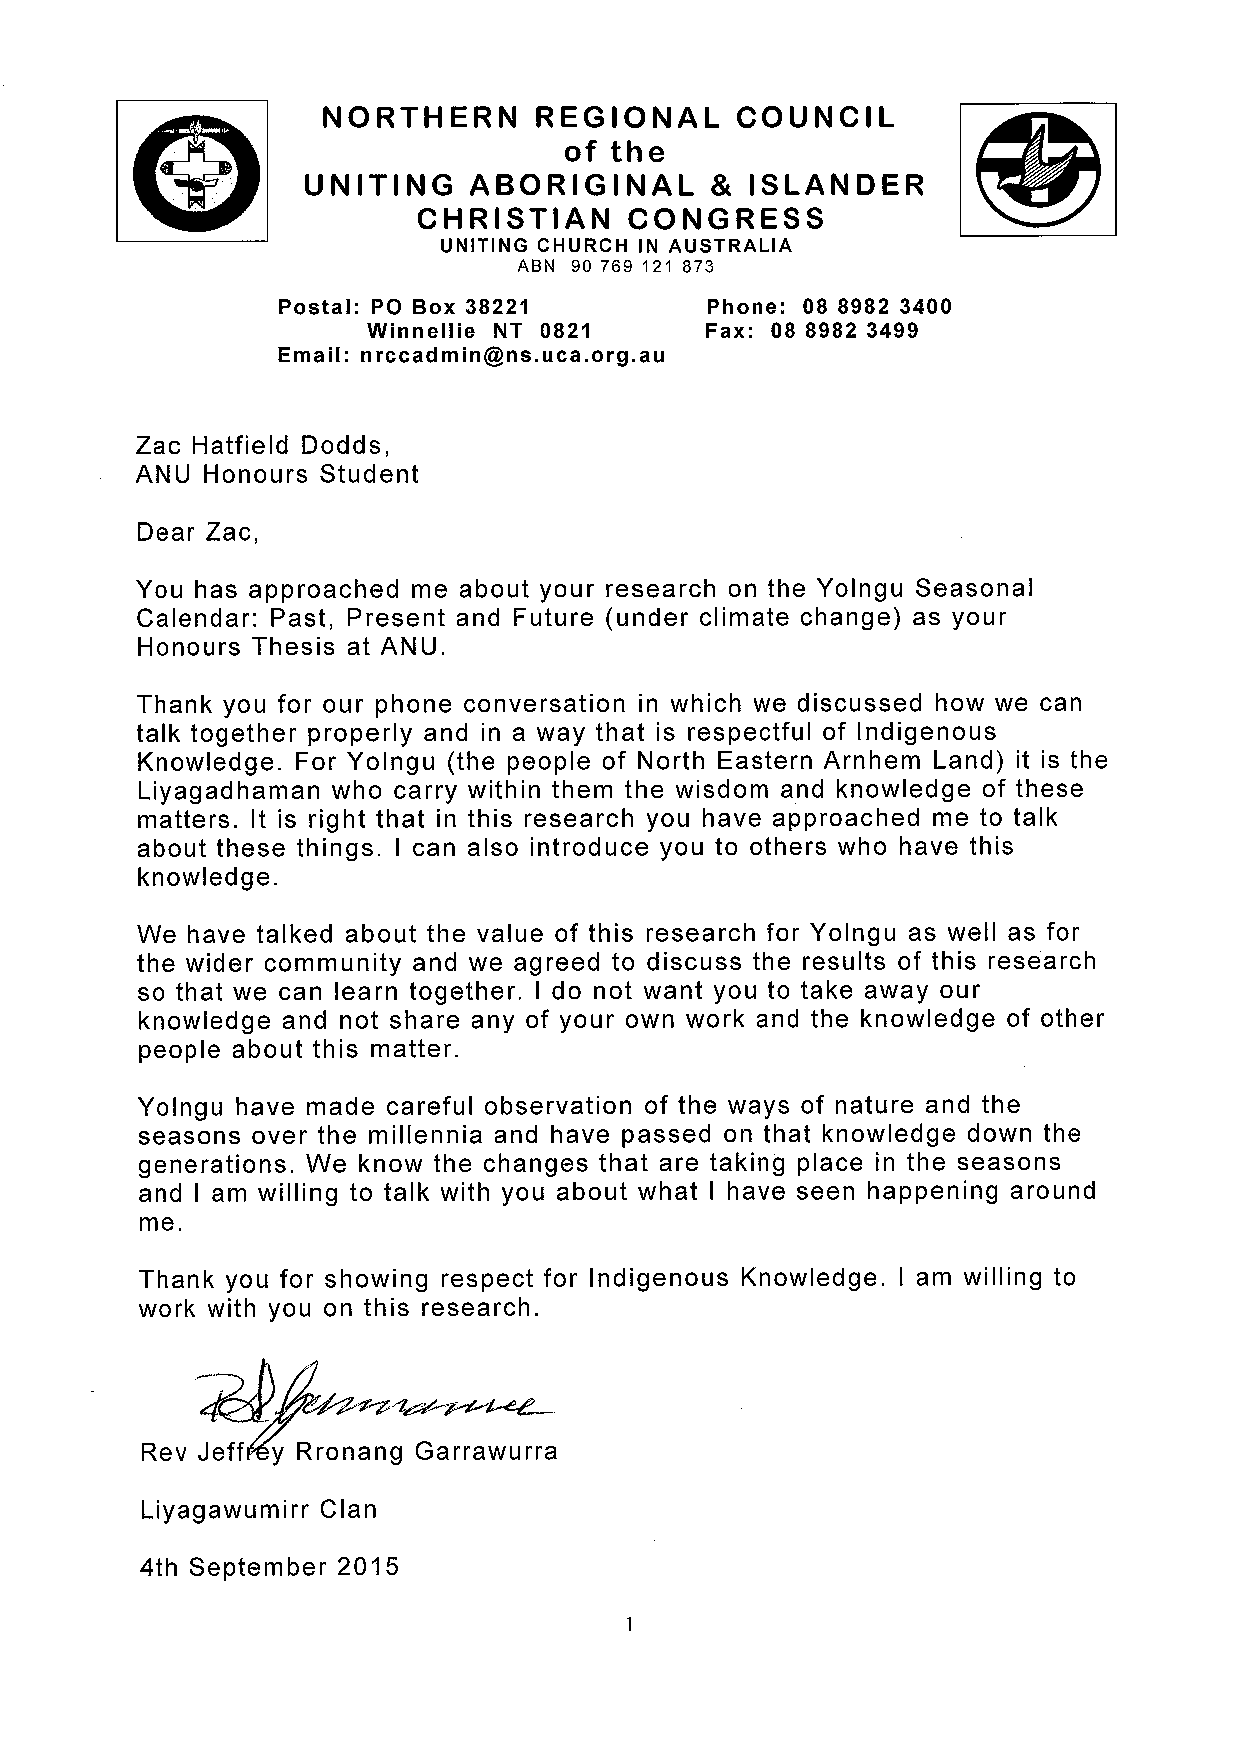
\includegraphics[width=0.9\textwidth]{invitation-letter.pdf}}
    \caption[Letter of invitation for collaborative research]{
        The formal invitation to study Yolngu seasons,
        and share results with both first and second peoples.
        Pre-existing relationships, with Yolngu and non-indigenous people,
        were essential in arranging this collaboration.
        }
    \label{app:invitation-letter}
\end{figure}


\section{Code and Data} \label{sec:appendix-code}
All the code and data I used are included in the supplementary material,
attached as electronic appendices.  Additional copies available on request.

To ensure long-term preservation of the electronic appendices, they
are provided as a .zip archive with the following SHA1 checksum:

da39a3ee5e6b4b0d3255bfef95601890afd80709

(that's the hash of an empty string, as the archive mentioned doesn't exist yet)



\section{Further Figures}
This section contains figures which would unnecessarily disrupt the
flow of the thesis, but should not be left to the electronic appendices.

\begin{figure}[p]
    \centering
    \includegraphics[width=\textwidth]{galiwinku/seabreeze-direction.pdf}
    \caption[3-hourly wind direction heatmaps, Galiwinku]{
        3-hourly wind direction heatmaps for Galiwinku,
        showing the northerly sea-breeze in the afternoon.
        Based on this figure, I judged that the difference between
        3pm and 6pm wind for season detection is small enough that
        I prefer the meteorological standard (3pm) over Yolngu advice (6pm).}
    \label{fig:galiwinku-seabreeze-direction}
\end{figure}
